\documentclass{article}
\PassOptionsToPackage{dvipsnames}{xcolor}
\usepackage{arxiv}

\usepackage[utf8]{inputenc} % allow utf-8 input
\usepackage[T1]{fontenc}    % use 8-bit T1 fonts
\usepackage[hidelinks]{hyperref}       % hyperlinks
\usepackage{url}            % simple URL typesetting
\usepackage{booktabs}       % professional-quality tables
\usepackage{amsmath,amssymb,amsthm}
\usepackage{amsfonts}       % blackboard math symbols
\usepackage{nicefrac}       % compact symbols for 1/2, etc.
\usepackage{makecell}
\usepackage{microtype}      % microtypography
\usepackage{mathrsfs}
\usepackage{float}
\usepackage{graphicx}
\usepackage{doi}
\usepackage{acronym}
\usepackage{listings}
\usepackage{siunitx}
\usepackage{tabularx}
\usepackage{tikz}
\usepackage[dvipsnames]{xcolor}

\usetikzlibrary{trees}

\def\checkmark{\tikz\fill[scale=0.4](0,.35) -- (.25,0) -- (1,.7) -- (.25,.15) -- cycle;}
\def\cross{\tikz\draw[scale=0.3, black, line width=0.3mm](0,0) -- (1,1) -- (0.5,0.5) -- (0,1) -- (1,0) -- (0.5,0.5);}

\newacro{abm}[ABM]{Agent-Based Model}
\newacro{cabm}[CABM]{Cellular Agent-Based Model}
\newacro{ca}[CA]{Cellular Automaton}
\newacro{ib}[IB]{Individual-Based}
\newacroplural{ca}[CA]{Cellular Automata}
\newacro{cpm}[CPM]{Cellular Pottes Model}
\newacro{ecoli}[\textit{E.coli}]{\textit{Escherichia coli}}
\newacro{bsubtilis}[\textit{B.subtilis}]{\textit{Bacillus subtilis}}
\newacro{spombe}[\textit{S.pombe}]{\textit{Schizosaccharomyces pombe}}
\newacro{paeruginosa}[\textit{P.aeruginosa}]{\textit{Pseudomonas aeruginosa}}
\newacro{pg}[PG]{peptidoglycan}

\newcommand{\todo}[1]{\colorbox{WildStrawberry}{\textcolor{white}{#1}}}

\newcommand{\R}{\mathbb{R}}

\title{Spatial Models of Rod-Shaped Bacteria - From Single-Cell Essays to Collective Phenomena}

%\date{September 9, 1985}	% Here you can change the date presented in the paper title
%\date{} 					% Or removing it

\author{
    \href{https://orcid.org/0009-0001-0613-7978}{
        
\includegraphics[scale=0.06]{orcid.pdf}
        \hspace{1mm}Jonas Pleyer
    }
    \thanks{
        \href{https://jonas.pleyer.org}{jonas.pleyer.org},
        \href{https://cellular-raza.com}{cellular-raza.com}
    }\\
	Freiburg Center for Data-Analysis and Modeling\\
	University of Freiburg\\
	% \texttt{jonas.pleyer@fdm.uni-freiburg.de} \\
	\And
    \hspace{1mm}Toquinha-Orelia Bergmann\\
	Freiburg Center for Data-Analysis and Modeling\\
	University of Freiburg\\
	%% examples of more authors
	\And
	\href{https://orcid.org/0000-0002-6371-4495}{
        
\includegraphics[scale=0.06]{orcid.pdf}
        \hspace{1mm}Christian Fleck
    }\\
	Freiburg Center for Data-Analysis and Modeling\\
	University of Freiburg
}

% Uncomment to remove the date
%\date{}

% Uncomment to override  the `A preprint' in the header
\renewcommand{\headeright}{Preprint}
%\renewcommand{\undertitle}{Technical Report}
\renewcommand{\shorttitle}{Spatial Models of Rod-shaped Bacteria}

\usepackage{enumitem}
\setlist{nolistsep}

%%% Add PDF metadata to help others organize their library
%%% Once the PDF is generated, you can check the metadata with
%%% $ pdfinfo template.pdf
\hypersetup{
pdftitle={Spatial Models of Rod-shaped Bacteria},
pdfsubject={q-bio.NC, q-bio.QM},
pdfauthor={Jonas Pleyer, Christian Fleck},
pdfkeywords={},
}

% Change numbering of equations
% \numberwithin{equation}{section}

\begin{document}
\maketitle

% TABLE OF CONTENTS
% Remove this before submission

%###################################################################################################
\begin{abstract}
    % \begin{itemize}
    %     \item Rod-shaped bacteria are everywhere
    %     \item many different species
    %     \item Shape plays crucial role in many effects such as motility, growth, collective effects etc.
    %     \item How does the behaviour of individual cells lead to collective phenomena?
    %     \item Mathemtical models help us to understand this
    %     \item We provide review of current state
    %     \item question; which biological required? answer: mesoscopic; want to get to emergent
    %         collective phenomena from single-cell behaviour
    % \end{itemize}
    Rod-shaped bacteria are ubiquitous forms of life which can be found in diverse microenvironments
    encompassing a wide, diverse range of species.
    Their elongated shape plays a crucial role in many biological processes such as enhancing
    swimming capabilities or promoting surface interactions.
    A key question is how the individual behaviour of multiple bacteria can lead to emergent
    spatial phenomena such as swarming and biofilm formation.
    Mathematical and computational methods provide powerful tools which allow researchers to bridge
    this gap and analyze the impact of various single-cell processes systematically.
    In this review we capture the current state of mathematical and computational approaches,
    emphasizing flexible, mesoscopic models which can be adjusted to describe a wide range of
    biological processes at their respectively required level of detail in order to study a variety
    of collective effects.
    We come to the conclusion that mechanical properties have been investigated extensively while
    other biolgical effects such as extracellular signalling, growth and differentiation are less
    studied.
\end{abstract}

% keywords can be removed
\keywords{Spatial \and Modeling \and Rod-Shaped \and Bacteria \and Mathematics}

% \textbf{POSSIBLE TITLES}
% \begin{itemize}
%     \item Mechanical Models of Rod-Shaped Bacteria - From Single-Cell Modeling to Collective Phenomena
%     \item Mathematical Modeling of Rod-Shaped Bacteria - From Single-Cell Mechanics to Collective Phenomena
%     \item Mathematical Models of Rod-Shaped Bacteria - From Single-Cell Analyses to Collective Phenomena
% \end{itemize}

\vfill
\pagebreak
\tableofcontents
\vfill
\pagebreak

%###################################################################################################
\section{Introduction}

\begin{itemize}
    \item Interested in all variations of rod-shaped bacteria; stiff, flexible, spiral, etc.
    \item Einordnung in andere Bakterienarten
    \item Rods are "more fundamtenal" than spheres (cocci) (which citation?)
    \item mesoscopic approach; take what cellular behaviour we need; interested in multicellular
        dynamics ultimately
    \item Talk about differences between: Gram-Positive, Gram-Negative
    \item Morphologies: Bacilli, Corkscrew, Filamentous, Spirochete
\end{itemize}

Order of this review
\begin{enumerate}
    \item Describe Biological Reality of Rod-shaped bacteria; single-cell; emergent phenomena
    \item What do we need within a model?
    \item Discuss modeling approaches; Mathematical, Computational
    \item Compare reusable computational tools
    \item Can we estimate their parameters?
\end{enumerate}

\section{Biological Principles - sorted}
\subsection{Cellular Properties}

\todo{move this to introduction}
Bacteria, unicellular divers procaryotic organisms and one of the simpler model to study individual single cell morphogenic changes up to emergent spatial emergent phenomena \cite{Vollmer2001}.
Various cell shapes are encountered in the prokaryotic world/Contain cells of different shapes, and yet we know little about how these shapes affect community biology \cite{Smith2017}.

Among the Well-studied examples include rod-shaped bacteria. Including gram negative as well as gram positive bacteria \ac{ecoli} (a Gram-negative bacterium) and \ac{bsubtilis} (Gram-positive) \cite{Chang2014}.

Including gram negative as well as gram positive bacteria \ac{ecoli} (a Gram-negative bacterium) and \ac{bsubtilis} (Gram-positive) \cite{Chang2014}.

\subsubsection{Cell shape}

\paragraph{Interplay of Cell Wall and Cytoskeleton}
\paragraph{Cell Wall}
\begin{itemize}
    \item \cite{Garner2021} "Toward a Mechanistic Understanding of Bacterial Rod Shape Formation and Regulation" \todo{why are we citing this?}
    \item \cite{Daniel2003} 2 ways maintaining rod shape: with/without MReB: A few rod-shaped bacteria have no MreB system.
        Different mechanism based on use of polar growth zones derived from the division machinery (\ac{pg} and FtsZ)
    \item \cite{Amir2014} bacterial cell shape is physically determined by the \ac{pg} cell wall
    \item \ac{pg} not sufficient for maintaining rod-shape on its own, need more effects \todo{do we need more details from this paper?} \todo{@Toqi find citation}
\end{itemize}
\paragraph{Cytoskeleton}
\begin{itemize}
    \item It was long believed that bacteria lack cytoskeletal filaments but with the end of the last century, it was discovered that the MreB protein fills this role since it "[..] forms an actin-like cytoskeleton in bacteria [..]" \cite{Erickson2001}.
    \item It can polymerize and form filaments which behave similar to actin microfilaments \cite{Dersch2020}.
    \item Studies of its crystal structure further showed the similarity to actin~\cite{vandenEnt2001} and the MreB, MreC and MreD proteins were identified as homologues of actin \cite{Lowe2017_lj}.
    \item \cite{Ausmees2003} extension to point before: Intermediate filaments (IFs) bacterial equivalent to IF proteins, named crescentin
    \item \cite{Bratton2018} role of "cytosceleton": MReB decides shape of bacteria
    \item \cite{vanTeeffelen2018} "Recent advances in understanding how rod-like bacteria stably maintain their cell shapes" \todo{@Toqi what can we learn from this citation?}
    \item \cite{Shi2018} \todo{remove this when done} points from book: Intracytoplasmic membranes,
        Membrane structure, Periplasm, Capsule, S-layer (surface layer)
\end{itemize}
\paragraph{Interplay}
\begin{itemize}
    \item \cite{Huan2021} Understanding \ac{pg} assembly and bacterial morphogenesis as well as de novo estabilshement of Cell Poles in gram-negative bacterium Myxococcus xanthus \todo{sort this somewhere}
\end{itemize}

\paragraph{Cells are flexible/filamentous, not always straight}

In bacteria the MreB protein forms an actin-like cytoskeleton~\cite{Erickson2001}.
It can polymerize and form filaments which behave similar to actin microfilaments~\cite{Dersch2020}.
The effect of MreB on the shape of cells during growth was shown in more detail
by~\cite{Ursell2014}.
They found that MreB localizes specifically at regions of negative curvature and thus introduces
heterogeneous cell growth which results in a bending force during the growth of cells.
It also means that the cells are able to sense the curvature of the cell wall through cytoskeleteal
MreB filaments during growth.
\cite{Bratton2018} showed that the trans-membrane protein RodZ can modulate MreB density and
facilitates local MreB assembly.
This feedback mechanism will result in straight rod-shaped bacteria if not interfered from the
external environment.
These results were also confirmed by the studies of~\cite{Wang2010}.
In their experiments, a single bacterium was fixed at the bottom pole while an optically trapped
bead was placed on the upper pole.
They could now exert a force on the free part and thus study the response of the cell under
different conditions.
When treating cells with \ac{a22},~\cite{IWAI2002,Gitai2005,Karczmarek2007,Bean2009}, a higher displacement with identical force
could be measured, thus indicating that MreB increases mechanical rigidity of the cell.

MReB also improtant/essential for actin-like MreB protein in bacterial chromosome segregation can be inhibited by A22 \cite{Gitai2005}A22 Disrupts the Bacterial Actin Cytoskeleton by Directly Binding and Inducing a Low-Affinity State in MreB \cite{Bean2009}


Furthermore \cite{Wachi1987} found that mutants of \ac{ecoli} which create defective MreB proteins will be spherical instead of their natural rod-shaped form.
A22, was found to induce spherical cells and spherical anucleate cells in E. coli. M, 22 induced a deep blue zone around a growth inhibitory zone, A22 was rel-atively ineŠective against Gram-positive bacteria - A22 induced spherical cell shapes in E. coli \cite{IWAI2002} 
rodZ deletion also forms spherical cell shapes \cite{Shiomi2008}
DNA and origin region segregation are not affected by the transition from rod to sphere after inhibition of Escherichia coli MreB by A22 \cite{Karczmarek2007}

% other species
This raises whether a rod shape serves any particular purpose.
It can be argued that the earliest cells consisted of "[..] rods and filaments with cocci being
derived and degenerate forms." \cite{Young2006} The Selective Value of Bacterial Shap.

\cite{Jones2001} studied the species of different bacterial sub-kingdoms which have the MreB gene.
They concluded: "Many of the organisms are rod shaped, similar to B. subtilis and E. coli.
Organisms with more complex shapes, including curved, filamentous, and helical bacteria, were all abundantly represented." \cite{Jones2001} (supplement: [p. 7]).

\cite{Zapun2008} "The different shapes of cocci"

The importance of shapes on the function of cells is highlighted by~\cite{Takeuchi2005} who grew
\ac{ecoli} in very narrow microchambers and thus permanently altered their shape.
This resulted in modified motion of the cells, some unchanged (helical and short crescent cells),
some dysfunctional (coiled cells).
It is important to note that this experiment controlled only the shape of bacteria without altering
any additional biochemical or genetic functions.

\subsubsection{Growth, Division and Regulation - intracellular}

\begin{itemize}
    \item \cite{DenBlaauwen2008} Nice paper about the molecular processes which are involved to maintain the shape of the rods
    \item MreB travels along the axis of elongation with a velocity that depends on the size of the filament \cite{Olshausen2013}. \todo{do we need this?}
\end{itemize}

\textbf{TODO look for other cell-division literature (specific to rods)} 
\cite{Lleo1990} "Bacterial cell shape regulation ..." \cite{Cooper1991}   growth of the gram-negative bacterial cell wall - cell surface during the division cycle 
Despite their differences in wall-thickness, \ac{bsubtilis} and \ac{ecoli} follow growth rules which are
comparable with respect to the extension of the rod \cite{Chang2014}.

Rod-shaped bacteria can grow by extending their circular part, such as \ac{ecoli} and ac{bsubtilis}~\cite{Errington2020} or by inserting new material at the tip of the rod.
The material is inserted in small bursts on the nanoscale in forms of patches, bands or hoops~\cite{DePedro2003} like \ac{spombe}.

\cite{Si2015} "Bacterial growth and form under mechanical compression" (push on cells; make them into flat disk-like structures; analyse growth)
\cite{Billaudeau2017} "Contrasting mechanisms of growth in two model rod-shaped bacteria"
\cite{Wang2010_2} "Robust Growth of Escherichia coli"

\cite{Bertrand2019} lag-phase in bacterial growth

\cite{Bramkamp2009} "Division site selection in rod-shaped bacteria"
\cite{Lan2007} "Z-ring force and cell shape during division in rod-like bacteria"
\cite{denBlaauwen2018} "Is Longitudinal Division in Rod-Shaped Bacteria a Matter of Swapping Axis?"
\cite{Koch1995} TODO "A physical basis for the precise location of the division site of rod-shaped bacteria: the Central Stress Model Free"


The importance of shapes on the function of cells is highlighted by~\cite{Takeuchi2005} who grew
\ac{ecoli} in very narrow microchambers and thus permanently altered their shape.
This resulted in modified motion of the cells, some unchanged (helical and short crescent cells),
some dysfunctional (coiled cells).
It is important to note that this experiment controlled only the shape of bacteria without altering
any additional biochemical or genetic functions.

\subsubsection{Nutrient uptake/distribution, Movement, pathogens and addaptation} %  Stiffness? here or by shape section?

As discussed previously, the major contributor which allows rod-shaped bacteria to grow an keep their shape is MreB.
If left alone, the rod will be straight but external effects can alter the morphology permanently~\cite{Takeuchi2005}.

\cite{Shen2022} "Bending stiffness characterization of Bacillus subtilis’ flagellar filament"

\textbf{[Note (Jonas)]} \textit{In principle, this stress will be dependent on the position inside the cell~\cite{Chatterjee1988}.}

Multiple efforts have been made in recent years to measure and analyze the bending properties of individual bacteria.
\cite{Amir2014_2} designed an experiment similar to \cite{Wang2010,Wang2010_protocol} but instead of optically trapped beads, a flow was used to apply a uniform force on the rod.
Their method is non-invasive and allows for larger force scales.
Cell-division was suppressed with SulA, thus altering the cellular biochemistry.
Since the cells grow continuously, a straight  hape was recovered in every case.
With these methods, they demonstrated that the bacteria "[..] exhibit two fundamentally different modes of deformations and recover from them" \cite{Amir2014_2}.
These modes are elastic in which the cell recovers immediately and plastic which requires growth to restore its morphology.
Short pulses of forces resulted in elastic  eformations from which the cell recovered immediately.
Plastic changes in morphology were only possible under longer periods of persistent force exertion.
Figure X(B) compares the angle  of deflection before and after the snap-back which occurs after turning off the flow.
The linear fit of 66 experimental results under varying conditions shows that both modes contribute to the behaviour of the cells.

\cite{Moreau2018} "collective gliding dynamics of ultra-long filamentous cyanobacteria"
\cite{BrettFinlay2014} bacteria stick to surfaces
\cite{Shah2022} Some rod-shaped bacteria glide on top of surfaces

movement:
Flavobacterium (phylum bacteroidetes) cell-surface adhesins and rotary motors, Myxococcus (phylum proteobacteria) soil-dwelling microbe both are rod shaped while Mycoplasma (phylum firmicutes) a wall-less bacterial parasites (flask shaped) do gliding (do not have flagelaten) \cite{Shrivastava2015}
More details to gliding Myxococcus with pili \todo{@Toqi find citation}
swimming \cite{Kong2014} often Flagella propeled \cite{Harshey2015}

TODO Nutrient uptake/distribution
TODO Adhesion/attachment to surfaces


Asynchrony in the growth and motility responses to environmental changes by individual bacterial cells \cite{Senkei2007}
movement with type-IV pili \cite{Ellison2021}
Myxococcus xanthus predation: an updated overview and movement by type-IV pili \cite{ContrerasM2024}
chemo taxis basics \cite{Nikita2009}

In addition, the flagella can play an important role in the direct adhesion between cells \cite{Haiko2013}. Thus it is not correct to blindly apply the results for adhesion to surfaces to the interactions between bacteria.

\cite{Li2025} citation from van-gogh bundles; also contains subsection about nutrient uptake

Myxococcus xanthus degrade their PG and form spherical spores - germination reconstruct their PG layer and regain their rod shape without relying on any preexisting structural template - sphere to rod \cite{Huan2021}

starvation-dependent and starvation-independent pathways of sporulation and produce structurally different spores \cite{Licking2000}
B. subtilis can divide asymmetrically during sporulation one cell differentiation process \cite{Barák2019}

Baceriophagen \cite{Duckworth2002}

\subsection{Cell-Cell interaction, differentiation, biofilms and emergent phenomena} %  Stiffness? here or by shape section?

TODO some bacterial have lifecycle citation for other than Myxococcus xanthus 

Quorum sensing
\cite{MorenoGmez2023} Quorum sensing as a mechanism to harness the wisdom of the crowds
\cite{Liu2025} Quorum Sensing: Not Just a Bridge Between Bacteria
\cite{Boyer2009} "Many factors other than cell density were shown to affect N-acyl-homoserine lactones accumulation and interfere with the QS signalling process." "This review aims to resent all factors interfering with the AHL-mediated signalling process, at the levels of signal production, diffusion and perception."

some bacteria can fuse to each other when they are long enough at close distance \cite{Kudryashev2011}
Biofilm dispersion and quorum sensing \cite{Solano2014}
multi-species biofilms the stretegies to avoid neighbors due to competition \cite{Rendueles2012}
Enhanced survival of multi-species biofilms under stress \cite{Wisnu2022}
extrazelluläre polymere Subs-tanzen (EPS) nur chemisches gefunden udn anwendungen....
- verlieren ihre flagelaten loosing their mobility/flagelaten in anqerob enviroment
cell "differentiation" when forming biofilms - \cite{Lopez2010}
Myxobacteria: Moving, Killing, Feeding, and Surviving Together \cite{Jose2016} e.g for task division

Division of task outside of biofilms -  also cell-cell communication, exrtem in cyanos



\paragraph{Text from Other paper}
A colony of bacteria is known to form biofilms (Dunne 2002). This strategy is is beneficial for the
survival of the collective as it allows it to harness growth factors and migrate when necessary and
also plays an important role in bacterial infections in the biomedical sector~\cite{Ong1999}.
The formation of biofilms is only possible due to the attractive nature of bacterial interactions
towards each other and surfaces (Berne et al. 2018). To analyze bacterial adhesion to surfaces,
\cite{vanLoosdrecht1989} investigated the interactions of various bacteria with negatively charged
polystyrene.
They found that the interaction is characterized by a low Gibbs energy of $(2 - 3)kT$ per cell
which can be described by a secondary minimum of the DLVO-theory~\cite{Verwey1947,Derjaguin1993}
which is relevant for distances $\geq\SI{1}{\nano\meter}$.
At these distances, the DLVO potential acts as a generic adhesive potential.
Particles which stay in the secondary minimum are held together but even weak interactions are
enough to redisperse them which means that this state is reversible.
When approaching closer distances, more intricate mechanisms come into play in which the
heterogeneity of the materials in question needs to be considered.
\cite{Hori2010} described bacterial adhesion as a “two-phase process including an initial,
instantaneous and reversible physical phase (phase one) and a time-dependent and irreversible
molecular and cellular phase (phase two)”.

All these considerations become even more intricate when interactions between bacteria are considered.
Gram-negative bacteria (eg. E.Coli) express outer membrane proteins (adhesins) which allow them to
attach to various hosts (Beachey 1981, Vaca et al. 2019).
In addition, the flagella can play an important role in the direct adhesion between
cells~\cite{Haiko2013}.
Thus it is not correct to blindly apply the results for adhesion to surfaces to the interactions
between bacteria.

Biofilms: an emergent form of bacterial life \cite{Flemming2016}

\paragraph{Toqis Sorting} ?

A colony of bacteria is known (not everone does/can from biofilms TODO find citations) to form biofilms~\cite{Dunne2002}.
This strategy is beneficial for the survival of the collective as it allows it to harness growth factors and migrate when necessary and also plays an important role in bacterial infections in the biomedical sector \cite{Ong1999}.
The formation of biofilms is only possible due to the attractive nature of bacterial interactions towards each other and surfaces \cite{Berne2018}.
To analyze bacterial adhesion to surfaces, \cite{vanLoosdrecht1989} investigated the interactions of various bacteria with negatively charged polystyrene.
They found that the interaction is characterized by a low Gibbs energy of $2-3kT$ per cell which can be described by a secondary minimum of the DLVO-theory \cite{Derjaguin1993,Verwey1947} which is relevant for distances $>=1nm$.
At these distances, the DLVO potential acts as a generic adhesive potential.
Particles which stay in the secondary minimum are held together but even weak interactions are enough to redisperse them which means that this state is reversible.
When approaching closer distances, more intricate mechanisms come into play in which the heterogeneity of the materials in question needs to be considered.
\cite{Hori2010} described bacterial adhesion as a "two-phase process including an initial, instantaneous and reversible physical phase (phase one) and a time-dependent and irreversible molecular and cellular phase (phase two)".

All these considerations become even more intricate when not considering interactions of bacteria with surfaces but bacteria with each other. Gram-negative bacteria (eg. \ac{ecoli}) express outer membrane proteins (adhesins) which allow them to attach to various hosts \cite{Vaca2019,Beachey1981}.


The overall attractive nature of the bacterial forces can be seen in the stress response to positive and negative compression of a colony in a confined space.
\cite{Trejo2013} studied the formation of macroscopic wrinkles when growing bacteria in a confined space.
They were able to model the strain and stress of the collection of bacteria which requires that cells are connected by a (to first order) spring-like force.
The developing wrinkles could then be described by a buckling instability.

\cite{Duvernoy2018} used laser techniques and force microscopy to investigate adhesion of individual \ac{ecoli} and \ac{paeruginosa} cells.
They found that the adhesion forces of the rods are polar, resulting in mechanical tension which in turn determines daughter cell arrangement.
They measured the size of the grown bacterial colonies, fitted ellipses to their shapes and found that adhesion and polar adhesion in particular resulted in a greater difference between the long and short axis of the fitted ellipse and thus a more oval shape rather than circular (WT).
Furthermore, they measured the critical value $N_(2D\/3D)$ where the colony grows into a second layer on top of the base layer.
It was shown by \cite{Grant2014} Figure X B), that the point of transition depends on the rigidity of the surrounding gel and \cite{Duvernoy2018} extended this analysis, showing that the critical value $N_(2D\/3D)$ depends on the adhesive strength and polarity of the interaction.
\cite{Grant2014} described the growing bacterial colony as a disc with radius $R$ which is pressed into the agarose slab.
The authors created a purposely-designed simulation in `C++` in order to model the effects of the gel on the collection of bacteria.
They approximated individual bacteria as multiple overlapping spheres which were linked by nonlinear springs such that their dynamics correspond to the Euler-Bernoulli dynamic beam theory \cite{HAN1999}.
The physical interaction potential between multiple bacteria and the surface was of the form

\begin{equation}
    F(\epsilon) = C E_b (d/2)^(2 - \beta) \epsilon^\beta
\end{equation}

where only repulsive effects were considered and no attractive forces which is justified by the already dense packing of the bacteria in the experiment.
The value $F$ is the magnitude of the force, $E_b$ is the effective Young modulus of the whole bacterium, $epsilon$ is the distance of overlap between two spheres and $d$ the diameter of the spheres.
Their model also accounts for friction between cells which is based on Amonton's laws (against the direction of movement, proportional to the magnitude of the normal force) \cite{Hutchings2021}.
In order to portray growth, new spheres were inserted and cells divided upon reaching a threshold.
In combining all these aspects, the authors have constructed an agent-based model which was able to produce the stacking behaviour they set out to describe.

\subsection{Emergent Phenomena and Self-Organization}

\begin{itemize}
    \item \cite{Nagarajan2022} TODO use contents of this review
    \item \cite{Ingham2008} TODO swarming and other nice effects
    \item \cite{Starru} TODO also swarming; also has very nice model for rod-shaped bacteria; I have
        not seen this anywhere else; very nice
    \item \cite{Stewart2005} "Aging and Death in an Organism That Reproduces by Morphologically
        Symmetric Division"
    \item \cite{Jin2020} "Influence of cell interaction forces on growth of bacterial biofilms"
    \item 
\end{itemize}

Although the developing wrinkles mentioned in the preceding section can be characterized as a form of collective self-organization, they require a confined space and would not be observable otherwise.
In most cases, rod-shaped bacteria grow in a medium separated enough such that they can freely extend in space.
\cite{vanGestel2015} explored how \ac{bsubtilis} migrates over a surface by forming multicellular structures.
The cells organize themselves into "van Gogh bundles" of cells which are tightly aligned in chains which then form filamentous loops.
This phenomenon occurs at the border of the bacterial colony and the migration is driven by two phenotypically different cell types \cite{Lpez2010}.
"[The authors] propose that surfactin-producing cells reduce the friction between cells and their substrate, thereby facilitating matrix-producing cells to form bundles" \cite{vanGestel2015}.
It has been shown that mutants which combine \textit{srfA} and \textit{eps} are able to outperform the wild-type when it comes to colony expansion \cite{Velicer2009}.
In their final stage, van Gogh bundles consist only of matrix-producing cells although they depend on surfactin-producing ones during their development.
\cite{vanGestel2015} also constructed an agent-based model to describe the observed effects.
Cells are modeled as straight lines in the shape of a filament by connecting their ends to each other.
They are initially placed horizontally at the bottom of the simulation domain In order to update to the next position, three mechanisms are involved: (1) Cell elongation (2) Cell division (3) Cell turning.
While the first two are rather self-explanatory, in the last step, a new spatial orientation of the cells is chosen in order to minimize the potential energy

\begin{equation}
    V = (\pi - \alpha_1)^2 + (\pi - \alpha_2)^2
\end{equation}

where $\alpha_1$ and $\alpha_2$ denote the angles to their respective neighbors.
By choosing the new orientation at random with probability $P=1-e^(k(V_c-V_n))$ (where $V_c,V_n$ are the current and new potential energies), the parameter $k$ symbolizes the bending rigidity.
Their analysis found that a high bending rigidity can play a more important role than the overall cell size, i.e.
the growth rate.
Concerning the complexity of their model, the authors noted: "We did not aim to accurately model the biophysical details of the growth of van Gogh bundles (parameterization of such a model would be impossible), but rather to make a simple phenomenological model to shape our intuition [..]" \cite{vanGestel2015}.
While the authors correctly assessed that the parametrization of such a model with just one particular experiment would be very difficult, multiple sources combined which treat individual aspects of each cellular aspect can yield enough information to meaningfully produce results.
\cite{Dong2022} showed that van Gogh bundles aid in the self-healing of bacterial colonies.
They observed that an artificially introduced cut heals better at lower curvatures, which corresponds to a higher rigidity of the ensemble being placed more towards the outer region of the triangular-shaped cut.
This work served as a precursor for a very recent study by \cite{Li2025} in which they picked up on the Agent-Based model.
Here, they investigated the interplay of nutrient depletion and multiple biofilms on the capacity to form van Gogh bundles.
Their model used linear growth on the cellular level which is only a first-order approximation to the experimentally observed exponential growth discussed previously.
Furthermore, no forces were calculated between the bacteria but a "shoving algorithm" (collision detection) moved the agents around such that collisions were avoided.
Based on the approach of \cite{vanGestel2015} they implemented cell-turning with.
But more significantly, they implemented a reaction-diffusion system

\begin{equation}
    \frac{\partial C_s}{\partial t} = D_n \nabla C_s + r_n
\end{equation}

where $\nabla$ is the gradient, $D_n$ the diffusion coefficient and $r_n$ is the nutrient sink or source.
More precisely, the nutrient sinks (sources) $r_n$ have to be located at the positions of cells.
If we assume a simplification to a point-like interaction with the external environment, we can write as

\begin{equation}
    \frac{\partial C_s}{\partial t} = D_n \nabla C_s  + \sum\limits_i u_i r_n (x_i) \delta(x-x_i)
\end{equation}

where the sum ranges over all cells $i=1..$ and each cell might have an individual exchange range $u_i$ located at position $x_i$ which is denoted by the well-known dirac delta-distribution $\delta(x-x_i)$.
The authors compared a single-biofilm system with a multi-biofilm system and showed that motile cells can convert into matrix-producing cells in a nutrient depleted system.
The authors show that spores in the case of a nutrient-depleted system

\section{Mathematical \& Computational Frameworks}

\subsection{Modeling Aspects}

\begin{figure}
    \centering
    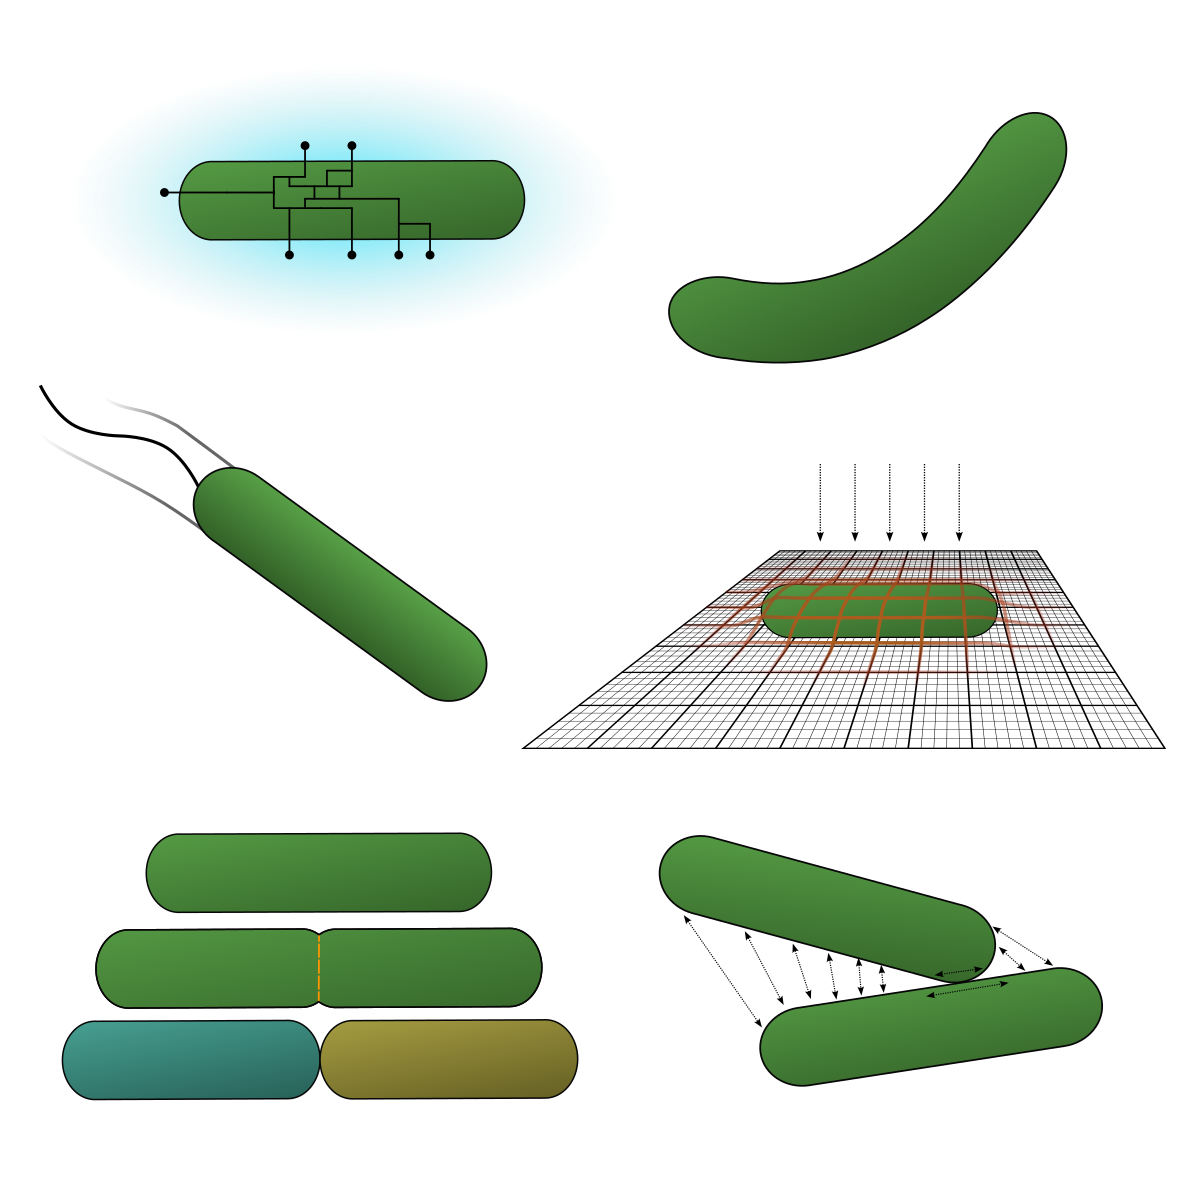
\includegraphics[width=0.5\textwidth]{figures/concept-figure.png}
    \caption{TODO}
    \label{fig:concept-figure-aspects}
\end{figure}

\begin{itemize}
    \item biological phenomena have been summarized before
    \item emphasize: more than just mechanics, also incorporate cell-cycle, extracellular
        reactions, (polar) interactions, etc.
    \item present "grouping" of biological phenomena into: (C) Cellular, (CC) Cell-Cell, (DC)
        Domain-Cell aspects \textbf{TODO possibly rename Domain to Environment}
    \item explain aspect-groups
    \item discuss table \ref{table:simulation-aspects}
\end{itemize}

\begin{table}[H]
    \newcounter{aspect}
    \setcounter{aspect}{1}
    \newcommand{\asp}{(\arabic{aspect}\refstepcounter{aspect})}
    \centering
    \def\arraystretch{1.3}
    \begin{tabularx}{\textwidth}{c l X}
        &\textbf{Aspect} & \textbf{Description}\\
        \toprule
        &\textbf{(C) Cellular}\\
        \midrule
        \asp & Rod-Shaped Mechanics &
            Rod-shaped bacteria are flexible rods which are able to freely move around (off-lattice
            approach) \cite{Takeuchi2005,Ursell2014,Amir2014_2}.\\
        \asp & Movement &
            \textbf{TODO} Flagellum, Swimming\\
        \asp & Growth &
            Cells grow exponentially by inserting new material either along the circular part of the
            rod or at the tip~\cite{Robert2014,Takeuchi2005}.\\
        \asp & Differentiation &
            \textit{B.subtilis} is known to differentiate into matrix-producing and
            surfactin-producing cells \cite{vanGestel2015,Lpez2010}.\\
        \asp & Division &
            The formation and continuation of van Gogh bundles is driven by cell division
            \cite{vanGestel2015}.
            Bacteria can form multilayers during their growth phase \cite{Duvernoy2018}.\\
        \asp & Variable Parameters &
            Parameters for individual cells are not fixed values but rather taken from a
            distribution \cite{Koutsoumanis2013}.\\
        &\textbf{(CC) Cell-Cell Interactions}\\
        \midrule
        \asp & Adhesion &
            Bacteria adhere to each other at longer distances and attach when in close contact
            \cite{Verwey1947,Trejo2013}.
            The interaction between rods can be polarized \cite{Duvernoy2018}.\\
        \asp & Friction &
            Friction between cells \cite{Grant2014} can be asymmetrical \cite{Doumic2020}.\\
        &\textbf{(DC) Domain-Cell Interactions}\\
        \midrule
        \asp & External Forces &
            Bacteria tend to stick to surfaces \cite{vanLoosdrecht1989}.
            The extracellular gel exerts a force onto the cells \cite{Grant2014}.\\
        \asp & Extracellular Reactions &
            Bacteria can take up nutrients or possible secrete/take up signalling molecules
            \cite{Li2025}.\textbf{TODO citation signalling}\\
        \bottomrule
    \end{tabularx}
    \label{table:simulation-aspects}
    \caption{TODO}
\end{table}

In order to describe the multicellular systems we looked at in the preceding sections, multiple
different aspects of cellular behaviour and their interactions with the surrounding domain need to
be considered and implemented.
Table \ref{table:simulation-aspects} summarizes these aspects and points to the relevant
experiments.
Aspects (1-5) take place inside the cell, (6,7) correspond to interactions between different
cellular agents and (8,9) to interactions with the domain.
It should be noted explicitly that these simulation aspects can be coupled to each other.
We have already seen such an example in the results of @Takeuchi2005 and @Ursell2014 where the
continued growth modulates the mechanical response of the cell.
Additionally, Aspect (5) is an overarching concept which is relevant for all processes.
Especially for the parameters which facilitate growth, we can assume that there is no direct
inheritance from one generation to the next but only a stochastic distribution of parameters from
which the new value is drawn (see supplement).

\subsection{Computational Modeling Frameworks}

\textbf{Frameworks}
\begin{itemize}
    \item \cite{breitwieser_biodynamo_2022} BioDynamo TODO mention this; I think no support
    \item \cite{Gorochowski2012,Matyjaszkiewicz2017} BSim; has rods
    \item \cite{Kreft1998,Kreft2001} (BacSim) "Individual-based modelling of biofilms Free"
    \item \cite{Kang2014} (Biocellion) only cylindrically-shaped potentials
    \item \cite{Gutirrez2017} \texttt{gro}
    \item \cite{Pleyer2025} \texttt{cellular\_raza}
    \item \cite{Bogdanowski2022} iDynomics \textbf{TODO check how this can model rods (it should)}
    \item \cite{GoiMoreno2015} DiSCUS \textbf{TODO}
    \item \cite{Li2019} NUFEB \textbf{TODO}
    \item \cite{Breitwieser2021} BioDynaMo \textbf{TODO}
    \item \cite{Dang2020} MultiCellSim \textbf{TODO}
    \item \cite{Hoehme2010} Tisim/CellSys \textbf{TODO}
    \item \cite{Grimm2006,Grimm2010} \textbf{TODO} "A standard protocol for describing individual-based and
        agent-based models" and update: \cite{Jang2012}
\end{itemize}

Since the beginning of this decade, multiple tools have emerged which are able to describe living
systems on a cellular individual-based approach in various details.
A good reason for choosing a framework over a purpose-built solution is to follow the Findability,
Accessibility, Interoperability and Reuse) FAIR principles by \cite{Wilkinson2016}.
These criteria have been designed to improve the overall infrastructure surrounding (re)usability of
scholarly data and methods.
In our previous work, we investigated their differences and features and capacity to model
individual behaviour of cells \cite{Pleyer2023}.
Using one of these existing toolkits means that already existing functionality can be used to
develop own models and the produced research results can be fed back to the library for fellow
researchers to reuse.
This begs the question, which of these existing models is able to support the long list of aspects
that we set out to describe with the experimentally gathered evidence.

\paragraph{Many general-purpose Frameworks lack explicit support for Rod-Shaped Bacteria}

\begin{itemize}
    \item \cite{Ghaffarizadeh2018} PhysiCell; no rods
    \item \cite{Swat2012} CompuCell; uses \ac{cpm}; no rods
    \item \cite{Cooper2020} Chaste; cell-centre and vertex-based; no rods
    \item \cite{Starru2014} Morpheus, uses \ac{cpm}; no rods
    \item \cite{Wei2013} BNSim; cells are spheres
\end{itemize}

Of the most popular frameworks, most do not support rod-shaped bacteria out of the box.
The very popular Cellular Potts Model (CPM) \cite{Graner1992} is mostly applied in 2D and only
represents cells as lattice grid points.
Since CompuCell3D \cite{Swat2012} exclusively builds upon the CPM, it can not model rod-shaped
bacteria.
PhysiCell \cite{Ghaffarizadeh2018} was designed to answer questions surrounding cancer research and
currently only supports spherical agents.
Chaste \cite{Cooper2020} was also designed for cancer research but further targets the heart and
tissues.
Naturally its Agent-Based Model supports cell-centre and vertex-based models but no rod shapes.
Morpheus \cite{Starru2014} also employs the CPM along with other spatial representations such as
vertex-based models or PDEs but has no support for Rod-Shaped bacteria.
Even purpose-built solutions such as BNSim \cite{Wei2013} which specifically targets bacterial
networks, assumes a simplified spherical representation for their bacterial agents.

\paragraph{Varying Support for Rod-Shaped Bacteria}

\begin{figure}[H]
    \centering
    \includegraphics[width=0.3\textwidth]{example-image-a}
    \includegraphics[width=0.3\textwidth]{example-image-b}
    \includegraphics[width=0.3\textwidth]{example-image-c}
    \caption{TODO: Snapshots of Modeling Frameworks}
\end{figure}

As we have seen, many frameworks do not provide existing functionality for rod-shaped bacteria.
However, some others do have various levels of support.
Biocellion \cite{Kang2014} can model agents with cylindrical interaction potentials but does not
model any of the MreB-related bending and rigidity or polar interactions.
They acknowledge this shortcoming: "Mapping a cell to multiple agents is also necessary to
separately model subcellular compartments [..].
However, Biocellion does not yet support this." \cite{Kang2014}
BSim2.0 represents cells as rigid capsular cells made from a cylindrical center part and two
half-spheres, which are placed at the ends of the cylinder to round out the shape.
In order to calculate interactions between cells, possible overlaps are determined and minimized,
thus determining the position values of the next iteration step.
It also accounts for many other phenomena, which are displayed in \textbf{TODO replace}.
BSim does not consider bending forces for individual cells or polar interactions.
The \texttt{gro} programming language was designed to simulate the growth of colonies and cell-cell
communication.
Its "physics computation has been optimized for rigid rod-shaped bodies, like E. coli bacteria"
\cite{Gutirrez2017}.
They recognize two types of forces which are acting on the cellular agents:
\textit{Local forces} which are calculated between adjacent bacteria and a \textit{global force}
which pushes bacteria outwards of the colony.
The latter of these is a phenomenological implementation of the observed colony expansion and the
associated central pressure with it.
This assumption may yield incorrect results for sparsely populated cases.
The engine is limited to 2D and does not consider polar interactions or bending of the rods.

\subsection{Purpose-Built Models}

\textbf{soft-matter keywords}
filamentous, nematic order

\textbf{include some references of soft-matter studies}
\begin{itemize}
    \item \cite{Duman2018} "Collective dynamics of self-propelled semiflexible filaments"
        (no division, no intracellular dynamics, no growth)
    \item \cite{Joshi2019} "The interplay between activity and filament flexibility determines the
        emergent properties of active nematics"
    \item \cite{Modica2024} "Soft confinement of self-propelled rods: simulation and theory"
    \item \cite{Peruani2006} "Nonequilibrium clustering of self-propelled rods"
    \item \cite{Saintillan2013} "Active suspensions and their nonlinear models" (suspensions of
        self-propelled microorganisms, dynamics of chemotactically responsive)
    \item \cite{Wensink2012} "Meso-scale turbulence in living fluids" (contains coarse-graining)
    \item \textbf{TODO look for more mixed-morphology (rods \& spheres) papers}
\end{itemize}

\textbf{Others}
\begin{itemize}
    \item \cite{Rosenberger1978} "Surface growth in rod-shaped bacteria" (Mathematical Model)
    \item \cite{Hsu2009} "A 3D Motile Rod-Shaped Monotrichous Bacterial Model" (Mathematical \&
        Numerical model for rigid rods which move with flagella)
    \item \cite{Hu2015} "swimming properties of an E. coli-type model bacterium are investigated by
        mesoscale hydrodynamic simulations"
    \item \cite{Cooper2006} "we conjecture that the current observed shape of these bacteria may
        have been determined, in part, to obtain the most efficient shape for moving through liquids."
    \item \cite{Schuech2019} \textbf{TODO study this in more detail} take into account curvature;
        have in-silico model
    \item \cite{Cylke2023} growth of \ac{ecoli} might be super-exponential; quantitative analysis of
        "morphogenetic noise"
\end{itemize}

\begin{itemize}
    \item \cite{Abar2017} "Agent Based Modelling and Simulation tools: A review of the state-of-art software"
    \item other generic frameworks exist, which may allow to model the desired functions
    \item \cite{Winkle2017} "Modeling mechanical interactions in growing populations of rod-shaped bacteria"
    \item \cite{Doumic2020} "A purely mechanical model with asymmetric features for early morphogenesis of
  rod-shaped bacteria micro-colony"
    \begin{itemize}
        \item This is a really good paper for referencing
        \item no bending in mathematical model
        \item Compare distributions of "Read-Outs" to data
        \item uses steric force (see also previously \cite{Trejo2013})
    \end{itemize}
    \item \cite{Grant2014} purposely-built model written in `C++`
    \begin{itemize}
        \item describes bacteria as collection of overlapping spheres
        \item spheres are coupled by non-linear springs (Euler-Bernoulli dynamic beam theory);
        This assumption is unfounded; they show however that it does not alter their results in this
        case
        \item only model repulsive forces; no attraction, adhesion
    \end{itemize}
    \item \cite{Cho2007} only 2D, no bending, no parameter estimation; based on work done in 
        \cite{Jnsson2005}
    \item \cite{Storck2014} TODO;
    41 Parameters for various cases;
    only 8 parameters taken from literature values/quantified;
    generated growth rate randomly (normal distribution), but for each growth step; this is
      stochastically equivalent but numerically slightly more intense;
    \item \cite{Volfson2008} TODO; continuum model, equations of nematodynamics \cite{Doi1988-ad}
    \begin{align}
        \partial_t \rho + \partial_z (\rho \nu) &= \alpha \rho\\
        \partial_t q + \nu \partial_z q &= B(1-q^2) \partial_z \nu\\
        \partial_t(\rho \nu) + \nu \partial_z (\rho \nu) &= - \partial_z p - \mu \rho \nu
    \end{align}
    \item \cite{Pleyer2023} TODO "Modeling mechanical interactions in growing populations of
        rod-shaped bacteria"
    \item \cite{Kong2014} TODO "Swimming motion of rod-shaped magnetotactic bacteria: the effects of
        shape and growing magnetic moment"
    \item \cite{Constantino2016} "Helical and rod-shaped bacteria swim in helical trajectories with
        little additional propulsion from helical shape"
    \item \cite{Starru} TODO very interesting FEM-based model
    \item \cite{Martins2015} "'miSimBa' — A simulator of synthetic time-lapsed microscopy images of
        bacterial cells"
    \item \cite{You2018} Hard-Rod model, continuous model
    \item \cite{Valdez2025} "Biomechanical modeling of spatiotemporal bacteria-phage competition"
\end{itemize}

\subsection{Parameter Estimation \& Techniques}

\textbf{Strategies for comparing simulation with data}
\begin{itemize}
    \item Simply do not compare: "Biolgically-inspired"
    \item Select specific feature to investigate
    \begin{itemize}
        \item Compare particular value (possibly with uncertainty)
        \item Compare multiple values
        \item Compare distribution
    \end{itemize}
    \item Fix some parameters from literature
    \item directly fit parameters from data (rare)
\end{itemize}

\textbf{Common Methods used for Analysis}
\begin{itemize}
    \item Cell-Segmentation~\cite{VanValen2016} omnipose~\cite{Cutler2022},
        cellpose~\cite{Stringer2020}
    \item Cell-Tracking 3DeeCellTracker \cite{Wen2021}; Comparisons of Tracking Algorithms
        \cite{Maka2014,Ulman2017}; Cell Tracking challenge \cite{Maka2023}
    \item Optimization method \textbf{TODO Citation}
    \item Profile-likelihood \cite{Kreutz2013}, structural/practical identifiability
        \cite{Heinrich2025}
\end{itemize}

\textbf{Papers which did some sort of parameter estimation}
\begin{itemize}
    \item \cite{Storck2014} TODO; 41 Parameters for various cases; only 8 parameters taken from
        literature values/quantified
    \item Highlight lack of estimation of mechanical parameters for Agent-Based Models
    \item \cite{Gallaher2017} TODO "Hybrid approach for parameter estimation in agent-based models"
    \item \cite{Nguyen2024} TODO tracking single cells; but then do bulk analysis with them, no
        rod-shaped bacteria
    \item \textbf{TODO add more of the soft-matter papers}
    \item \textbf{TODO see if any of the frameworks do have estimates}
\end{itemize}

\section{Discussion}

\begin{itemize}
    \item many details known from experimental/biological side
    \item missing link from individual-based behaviour to emergent phenomena
    \item Mainly discussed: \ac{ecoli}, \ac{bsubtilis} - list some species which have not been
        accounted for Bacillus licheniformis \textbf{TODO Find citation}
\end{itemize}

\section{Conclusion}

\begin{itemize}
    \item Large amount of biological processes that are relevant for spatial patterns
    \item Some studies which capture individual effects
    \item basically no framework that supports generalized model of rod-shaped bacteria
    \item many effects not studied; include more biology (cell-cycle, intra-/extracellular
        reactions, differentiation, cell-cell variability, etc.)
    \item comparison with experimental data lackluster
\end{itemize}

\bibliographystyle{IEEEtran}
\bibliography{references}

\renewcommand{\thesection}{}
\renewcommand{\thesubsection}{S\arabic{subsection}}

\section{Supplementary Material}
\subsection{Inheritance of Growth-Relevant Parameters}

We consider a distribution of parameters $rho(x)$ for
which the rate of proliferation of any cell is proportional to the value of the parameter $x$.
The rate of proliferation and thus the rate with which $rho(x)$ changes is given by
$partial_rho(x,t) x = lambda rho(x,t) x$.
This Ordinary Differential Equation (ODE) is trivially solvable with solution

\begin{equation}
    \rho(x,t) = \rho(x,t_0) \exp(\lambda t x)
\end{equation}

For the simple example of a Gaussian distribution
$\rho(x,t_0) = 1/\sqrt{2 pi \sigma^2} \exp(-x^2/(2 \sigma^2))$, we can calculate the expectation
value for the parameter $x$ via

\begin{align}
    E[x(t)]
    &= 1/\sqrt{2 \pi \sigma^2} \int \rho(x,t) x op("dx")\\
    &= 1/\sqrt{2 \pi \sigma^2} \int x \exp{-x^2/(2 \sigma^2} + \lambda t x) op("dx")\\
    % &= 1/sqrt(2 pi sigma^2) integral x exp( -(x - lambda sigma^2 t)^2/(2 sigma^2) - lambda^2 sigma^2 t^2) op("dx")\
    % &= 1/sqrt(2 pi sigma^2) integral x exp( -(x - lambda sigma^2 t)^2/(2 sigma^2) + (lambda^2 sigma^2 t^2) /2) op("dx")\
    % &= 1/sqrt(2 pi sigma^2) integral [- sigma^2 partial/(partial x) +lambda sigma^2 t] exp( -(x - lambda sigma^2 t)^2/(2 sigma^2))exp((lambda^2 sigma^2 t^2) /2) op("dx")\
    % &= 1/sqrt(2 pi sigma^2) integral lambda sigma^2 t exp( -(x - lambda sigma^2 t)^2/(2 sigma^2))exp((lambda^2 sigma^2 t^2) /2) op("dx")\
    &= \lambda \sigma^2 t \exp{(\lambda^2 \sigma^2 t^2)/2}.
\end{align}

We can see that the expected value $E[x(t)]$ keeps increasing faster than regular exponential growth
and indefinitely which is contrary to observation (see Figure \textbf{TODO}) and intuition.
The same qualitative result will emerge for different distributions.
With these considerations, we can assume that the new parameters of freshly divided cells are drawn
from a random distribution which carries no temporal correlation between the mother and daughter
cell. (TODO this should be provable more rigorously)
It has to be stated explicitly that these considerations were done under the assumption that the
proliferation of the cell is affected and proportional to the value of the parameter.

\end{document}
